\documentclass[12pt]{amsart}
\usepackage{amsaddr}
\usepackage{../marktext} 
%% Remove draft for real article, put twocolumn for two columns
\usepackage{../svmacro}
\usepackage[utf8]{inputenc}
\usepackage{lineno}
\usepackage[style=alphabetic, backend=biber]{biblatex}
\addbibresource{bibliography.bib}

%% commentary bubble
\newcommand{\SV}[2][]{\sidenote[colback=green!10]{\textbf{SV\xspace #1:} #2}}

%% Title 
\title{ MATH 102: Ideas  of Math }
\author{ Worksheet 1 }

\date{\today}

\begin{document}

\maketitle

If you are stuck, please don't look at the book for any of the question below during class.
Turn to your friends to discuss instead!

We are practicing reasoning without looking up the answer right away.
It is OKAY if you don't remember the solution.

\begin{question}
	Why do we prove things?
	What is the difference between mathematical proof and scientific proof?
\end{question}

\begin{question}
	Describe Sherlock's deduction to decide if the case is a murder or
	a suicide in the following clip:
	\url{https://www.youtube.com/watch?v=4PKr_BVo4hg}.

	Make sure to re-write in the premises and conclusion form as in the slides. Make sure you're as clear as you can so that the reader can see right away what're the premises and conclusion.
\end{question}


\begin{question}[8x8 chessboard]
	Can you fill the following chessboard with dominos?
	\begin{center}
		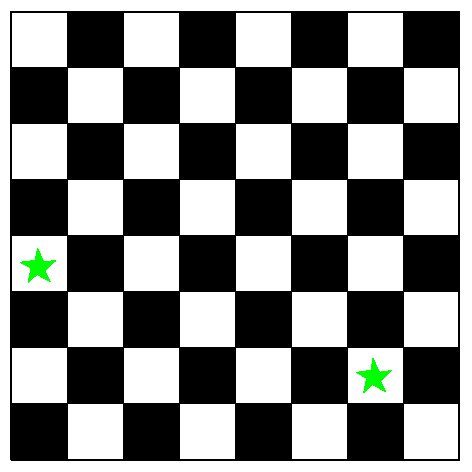
\includegraphics[width=0.5\textwidth]{Checker1.pdf}
	\end{center}

	How about this chessboard?
	\begin{center}
		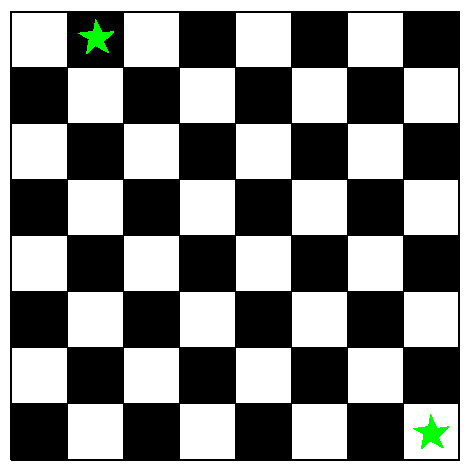
\includegraphics[width=0.5\textwidth]{Checker2.pdf}
	\end{center}
\end{question}

\begin{question}[10x10 chessboard]
	Can you fill the 10x10 chessboard with domino pieces that are twice as
	long as the normal domino piece?
	\begin{center}
		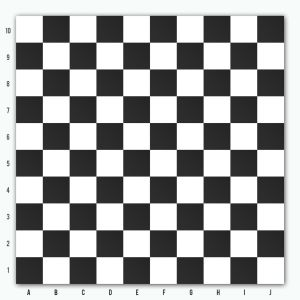
\includegraphics[width=0.6\textwidth]{Checker3.jpg}
	\end{center}
\end{question}

\begin{question}
	How many regions can you divide a disk into if you have $n$ points on the boundary?
	\begin{center}
		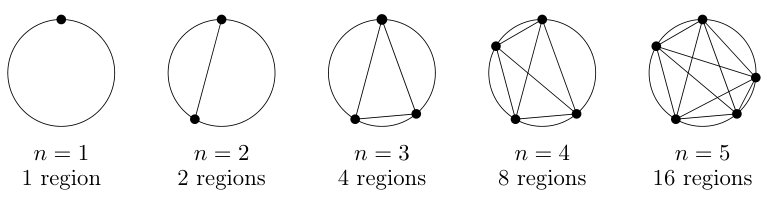
\includegraphics[width=0.8\textwidth]{Regions.png}
	\end{center}
\end{question}

\begin{question}
	\begin{enumerate}
		\item Discuss why Pigeonhole Principle (both simple and general forms) makes sense?
		      What information does it give? What information does it not give?
		\item Discuss why there are 3 people in Sacramento, CA, who have exactly the same number of hair.
	\end{enumerate}
\end{question}

\begin{question}
	\begin{enumerate}
		\item Give an estimate to see how many people may have the same birthday?
		\item Give an estimate to see how many people have the birthday on Wednesday?
		\item Whatt!!??
	\end{enumerate}
\end{question}

\begin{question}
	Suppose there are 10 marbles in a square of with side lengths of 3.
	Show that there are two marbles that are at most $\sqrt2$ apart.
\end{question}

\begin{question}[Hard]
	Given any 101 integers from $\{1, 2, 3, . . . , 200\}$, at least one of these numbers will divide another.
\end{question}

\printbibliography
%\bibliography{refs}
%\bibliographystyle{halpha-abbrv}


\end{document}
